\documentclass{article}
\usepackage[a4paper,left=3cm,right=3cm,top=3cm,bottom=3cm]{geometry}
\usepackage[utf8]{inputenc}
\usepackage[T1]{fontenc}
\usepackage{latexsym,amsfonts,amsmath,amssymb,amstext,graphicx,titlesec,ae,aecompl,mathtools,tabularx, multirow, cancel, nicefrac,subcaption, blindtext, floatrow}
\setlength{\parindent}{0pt}
\newfloatcommand{capbtabbox}{table}[][\FBwidth]


\begin{document}

\begin{titlepage}
       \begin{center}
             \begin{huge}
				   %% Update assignment number here
                   \textbf{Assignment 1}
             \end{huge}
       \end{center}

       \begin{center}
             \begin{large}
                   Computational Intelligence, SS2020
             \end{large}
       \end{center}

       \begin{center}
 \begin{tabularx}{\textwidth}{|>{\hsize=.33\hsize}X|>{\hsize=.33\hsize}X|>{\hsize=.33\hsize}X|} 

                   \hline
                   \multicolumn{3}{|c|}{\textbf{Team Members}} \\
                   \hline
                   Last name & First name & Matriculation Number \\
                   \hline
                   Blöcher & Christian & 01573246 \\
                   \hline
                   Bürgener & Max & 01531577 \\
                   \hline
                    &  &  \\
                   \hline

             \end{tabularx}
       \end{center}
\end{titlepage}

\section{Maximum Likelihood Estimation of Model Parameters}

\subsection{Which measurement in sc.2 is exponentially distributed?}

\begin{itemize}

    \begin{figure}[h]
        \centering
        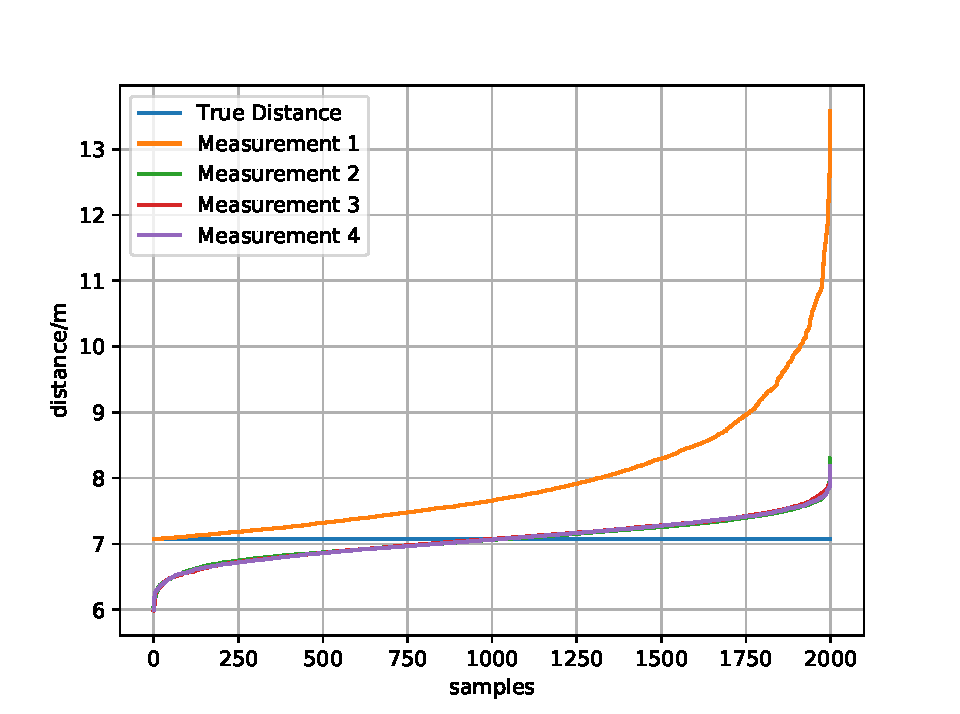
\includegraphics[width=\textwidth]{./Figures/scenario2_findexponential.pdf}
        \caption{Scenario 2 with mixed measurement models for the anchors}
        \label{fig:scenario2_findexponential}
    \end{figure}
    
    \item In figure \ref{fig:scenario2_findexponential} we can see that in scenario 2 the distance measurements from anchor 1 is exponentially distributed. It is the only distribution which is bigger than the true distance for all samples and its slope is rising exponentially for rising x-values.
    
\end{itemize}

\subsection{Derivation for the maximum likelihood solution
}
\begin{itemize}

    \item Analytical derivation for the Gaussian distribution:\\
  
	    $\begin{array}{ccc}
	        p(\tilde{d}_n(a_i,\mathbf{p})\mid\mathbf{p}) & = & \frac{1}{\sqrt{2\pi\sigma^2}} \cdot e^{- \frac{[\tilde{d}_n(a_i,\mathbf{p})-d(a_i,\mathbf{p})]^2}{2\sigma^2}} \\  
	    \end{array}$\\
	    
	    The data is independent identically distributed (iid), therefore the likelihood function is the product of all individual likelihoods\\
	    
	    $\begin{array}{ccc}
	        P(\tilde{d}_n(a_i,\mathbf{p})\mid\mathbf{p}) & = & \displaystyle \prod_{n=0}^{N-1} \frac{1}{\sqrt{2\pi\sigma^2}} \cdot e^{- \frac{[\tilde{d}_n(a_i,\mathbf{p})-d(a_i,\mathbf{p})]^2}{2\sigma^2}} \\

	    \end{array}$\\
	  
	    To convert the product to a sum we apply the natural logarithm.\\
	  
	    $\begin{array}{cccl}
	        L(\tilde{d}_n(a_i,\mathbf{p})\mid\mathbf{p}) & = & ln \left[ \displaystyle \displaystyle \prod_{n=0}^{N-1} \frac{1}{\sqrt{2\pi\sigma^2}} \cdot e^{- \frac{[\tilde{d}_n(a_i,\mathbf{p})-d(a_i,\mathbf{p})]^2}{2\sigma^2}} \right] & \\\\
	        L(\tilde{d}_n(a_i,\mathbf{p})\mid\mathbf{p}) & = & \displaystyle \sum_{n=0}^{N-1} \left[ ln(\frac{1}{\sqrt{2\pi\sigma^2}}) - \frac{[\tilde{d}_n(a_i,\mathbf{p})-d(a_i,\mathbf{p})]^2}{2\sigma^2} \right] & \\
	    \end{array}$\\
	  
	    Since we want to find the parameter $\sigma^2$, which maximizes the probability of the distance, we derive $L(\tilde{d}_n(a_i,\mathbf{p})\mid\mathbf{p})$ and set it to zero. \\
	
	    $\begin{array}{cccr}
	        L(\tilde{d}_n(a_i,\mathbf{p})\mid\mathbf{p}) & = & \displaystyle \sum_{n=0}^{N-1} \left[ ln(1) - \frac{1}{2}ln(2\pi\sigma^2) - \frac{[\tilde{d}_n(a_i,\mathbf{p})-d(a_i,\mathbf{p})]^2}{2\sigma^2} \right] & \mid \frac{\partial}{\partial\sigma^2} \\\\
	        \frac{\partial}{\partial\sigma^2} L(\tilde{d}_n(a_i,\mathbf{p})\mid\mathbf{p}) & = & \displaystyle \sum_{n=0}^{N-1} \left[ - \frac{1}{\sigma^2} + \frac{[\tilde{d}_n(a_i,\mathbf{p})-d(a_i,\mathbf{p})]^2}{\sigma^4} \right] & \stackrel{!}{=} 0 \\\\
	        0 & = & \displaystyle \sum_{n=0}^{N-1} \left[ - \frac{1}{\sigma^2} + \frac{[\tilde{d}_n(a_i,\mathbf{p})-d(a_i,\mathbf{p})]^2}{\sigma^4} \right] & \\\\
	        \frac{N}{\sigma^2} & = & \displaystyle \sum_{n=0}^{N-1} \frac{[\tilde{d}_n(a_i,\mathbf{p})-d(a_i,\mathbf{p})]^2}{\sigma^4} \\\\
	        \sigma^2 & = & \frac{\displaystyle \sum_{n=0}^{N-1}[\tilde{d}_n(a_i,\mathbf{p})-d(a_i,\mathbf{p})]^2}{N} 
	    \end{array}$\\
         	 
	\item Analytical derivation for the Exponential distribution:\\
	 
	    \begin{equation*}
	  	     p(\tilde{d}_n(a_i,\mathbf{p})\mid\mathbf{p}) = 
	         \begin{cases}
	             \lambda_i e^{-\lambda_i [\tilde{d}_n(a_i,\mathbf{p}) - d(a_i,p)]} & \quad \text{, }\tilde{d}_n(a_i,\mathbf{p}) \geq d(a_i,\mathbf{p}) \\
	             0 & \quad \text{, else}
	         \end{cases}
	     \end{equation*}
	    
            	         
	     $\begin{array}{cccl}
	         L(\tilde{d}_n(a_i,\mathbf{p}) \mid \mathbf{p}) & = & \displaystyle \sum_{n=0}^{N-1} ln(\lambda_i) - \lambda_i [\tilde{d}_n(a_i,\mathbf{p}) - d(a_i,\mathbf{p})] & \mid \frac{\partial}{\partial\lambda_i} \\\\
	         \frac{\partial}{\partial\lambda_i} L(\tilde{d}_n(a_i,\mathbf{p}) \mid \mathbf{p}) & = & \frac{N}{\lambda_i} - \displaystyle \sum_{n=0}^{N-1}[\tilde{d}_n(a_i,\mathbf{p}) - d(a_i,\mathbf{p})] & \stackrel{!}{=} 0 \\\\
	         \frac{N}{\lambda_i} & = & \displaystyle \sum_{n=0}^{N-1} [\tilde{d}_n(a_i,\mathbf{p}) - d(a_i,\mathbf{p})] & \\\\
	         \lambda_i & = & \frac{N}{\displaystyle \sum_{n=0}^{N-1} [\tilde{d}_n(a_i,\mathbf{p}) - d(a_i,\mathbf{p})]} & ,\tilde{d}_n(a_i,\mathbf{p}) \geq d(a_i,\mathbf{p})
	     \end{array}$\\
	 
\end{itemize}


\section{Estimation of the Position}
\subsection{Least-Squares Estimation of the Position}

\begin{itemize}
    \item Analytical conversion of the ML estimation equation:\\
    
        $\begin{array}{ccccl}
        	\hat{\mathbf{p}}_{ML}(n) & = & \underset{\mathbf{p}}{\textrm{argmax}} \displaystyle \prod_{i=0}^{N_A-1} p(\tilde{d}_n(a_i,\mathbf{p})\mid\mathbf{p}) & &\\
        	\hat{\mathbf{p}}_{ML}(n) & = & \underset{\mathbf{p}}{\textrm{argmax}} \;ln \left[ \displaystyle \prod_{i=0}^{N_A-1} p(\tilde{d}_n(a_i,\mathbf{p})\mid\mathbf{p}) \right] & &\\        
        	\hat{\mathbf{p}}_{ML}(n) & = & \underset{\mathbf{p}}{\textrm{argmax}} \displaystyle \sum_{i=0}^{N_A - 1} ln \left( \frac{1}{\sqrt{2\pi\sigma_i^2}}\right) - \frac{[\tilde{d}_n(a_i,\mathbf{p})-d(a_i,\mathbf{p})]^2}{2\sigma_i^2} & &\\
        \end{array}$ \\
       
        Because in scenario 1 we only use Gaussian models for all anchors that were calibrated with the same distance to the reference position, we can assume that $\sigma_i^2 = \sigma^2 \; \forall i$. That means the $ln$-term can be neglected since it only shifts the value of the maximum by a constant but does not affect its position. Similarly $\frac{1}{2\sigma^2}$ can be omitted, as it is also just a scaling factor. Furthermore $ \underset{\mathbf{p}}{\textrm{argmax}}\;(- \dots)$ is equivalent to $\underset{\mathbf{p}}{\textrm{argmin}}\;(\dots)$. Thus: \\
        
        $\begin{array}{ccccl}
        
        	\hat{\mathbf{p}}_{ML}(n) & = & \underset{\mathbf{p}}{\textrm{argmin}} \displaystyle \sum_{i=0}^{N_A-1} [\tilde{d}_n(a_i,\mathbf{p})-d(a_i,\mathbf{p})]^2 & = & \hat{\mathbf{p}}_{LS}(n)
        	    	
        \end{array}$
                 	
\end{itemize}



\subsection{Gauss-Newton Algorithm for Position Estimation}

\begin{itemize}

	\item Analytical solution for the Jacobian matrix.\\
	
	    $\begin{array}{ccc}
    
        \left[ J(p)\right]_{i,1} & = & \frac{\partial}{\partial x} \left[ \tilde{d}_n(a_i,\mathbf{p}) - \sqrt{(x_i - x)^2 + (y_i - y)^2} \right] \\\\
        \left[ J(p) \right]_{i,1} & = & -\frac{[(-)2(x_i-x)]}{2 \cdot\sqrt{(x_i - x)^2 + (y_i - y)^2}} \\\\
        \left[ J(p) \right]_{i,1} & = & \frac{(x_i-x)}{\sqrt{(x_i - x)^2 + (y_i - y)^2}}\\\\\\
        
        
        \left[ J(p) \right]_{i,2} & = & \frac{(y_i-y)}{\sqrt{(x_i - x)^2 + (y_i - y)^2}}\\\\\\

    \end{array}$


    \item Mean and variance

        \begin{table}[h]
        \centering
        \begin{tabular}{l||c||c|c||c|}
            \cline{2-5}
                                                       & \multirow{2}{*}{Scenario 1} & \multicolumn{2}{c||}{Scenario 2}                      & \multirow{2}{*}{Scenario 3} \\ \cline{3-4}
                                                       &                             & with exponential anchor & without exponential anchor &                             \\ \hline\hline
            \multicolumn{1}{|l||}{Error mean $\mu_{e}$}          & 0.278                      & 0.640                  & 0.399                     & 1.265                      \\ \hline
            \multicolumn{1}{|l||}{Error variance $\sigma^2_{e}$} & 0.022                      & 0.275                  & 0.054                     & 0.939                      \\ \hline
        \end{tabular}
        \caption{Error-mean and -variance for different Scenarios.}
        \label{tab:ls_mean_var}
        \end{table}
        
    Table \ref{tab:ls_mean_var} shows that the Gaus-Newton Algorithm is optimized for Gauss distributions. Mean $\mu_{e}$ and variance $\sigma^2_{e}$ are much bigger in the mixed scenario 2 and in scenario 3 which consists of 4 exponential distributions.
        
    \newpage
    
    \item Multivariate Gaussian distributions\\        
  
        \begin{figure}[hbt!]
        \begin{floatrow}
        \ffigbox{%
        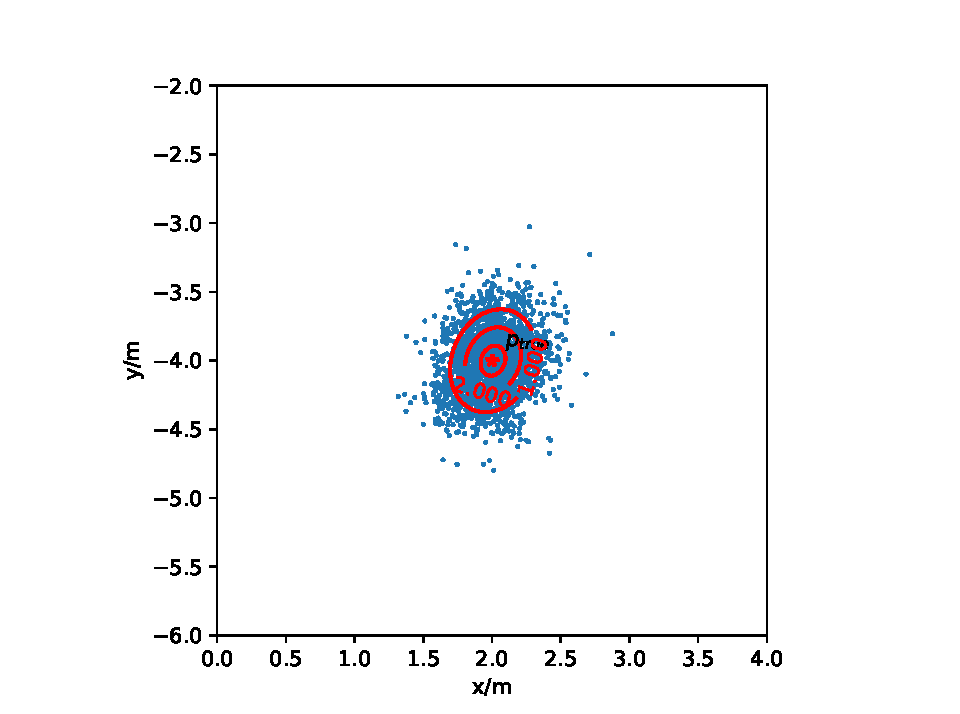
\includegraphics[width=.5\textwidth]{./Figures/scenario1_gausscont_big.pdf}
        }{%
        \caption{Gaussian distribution of scenario 1}%
        \label{fig:scenario1_gausscont_big}
		}
		\capbtabbox{%
  		\begin{tabular}{c|c} 
  		0,04603 & 0,00869 \\ \hline
  		0,00869 & 0,05823 \\ 
 		 \end{tabular}
		}{%
 		\caption{Covariance matrix}%
		}
		\label{tab:scenario1_covariance}
		\end{floatrow}
		\end{figure}
		
		The Gaussian distribution is computed by the Covariance matrix which is next to Figure \ref{fig:scenario1_gausscont_big}. The distribution for scenario 1 is almost \textit{spherically shaped} due to the small difference in the main diagonal and the very low values in the secondary diagonal. 
		
		\begin{figure}[hbt!]
        \begin{floatrow}
        \ffigbox{%
        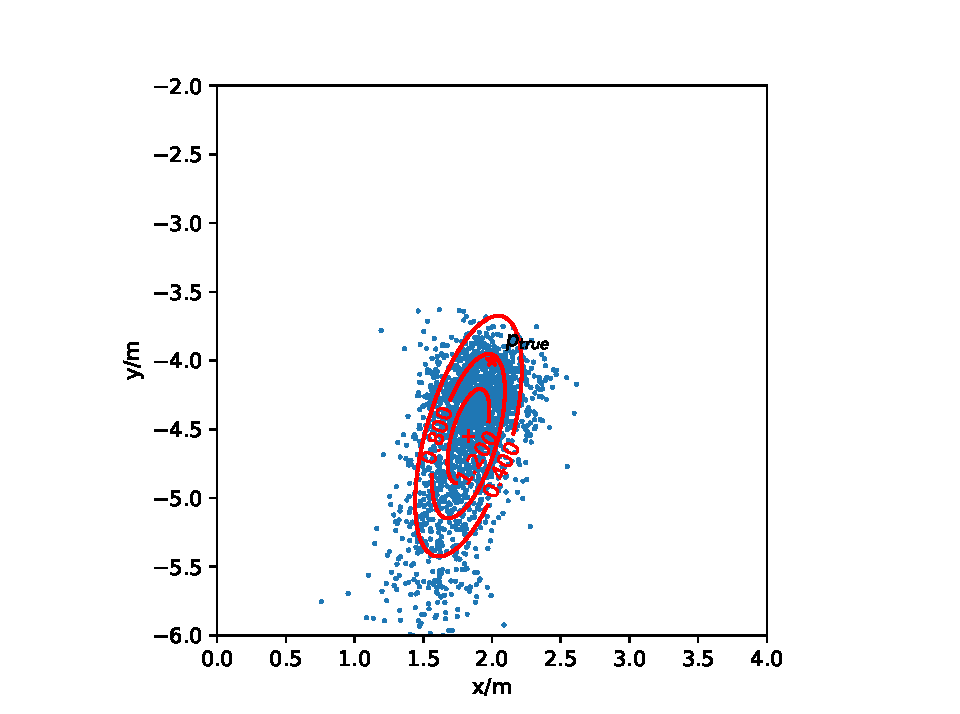
\includegraphics[width=.5\textwidth]{./Figures/scenario2_gausscont_big_withexp.pdf}
        }{%
        \caption{Gaussian distribution of scenario 2}%
        \label{fig:scenario2_gausscont_big_withexp}
		}
		\capbtabbox{%
  		\begin{tabular}{c|c} 
  		0,05783 & 0,07271 \\ \hline
  		0,07271 & 0,29491 \\ 
 		\end{tabular}
		}{%
 		\caption{Covariance matrix}%
		}
		\end{floatrow}
		\end{figure}
		
		With rising covariance values the variance around the mean value is rising. Therefore we can see a general Gaussian distribution in Figure \ref{fig:scenario2_gausscont_big_withexp} with the distribution stretched out in the direction leading away from the exponentially modelled anchor. That is because the exponentially distributed distance measurements are prone to take larger values than the Gaussian ones (s. figure \ref{fig:scenario2_findexponential}). This makes the position estimation less precise.
		
		\newpage
		
		\begin{figure}[hbt!]
        \begin{floatrow}
        \ffigbox{%
        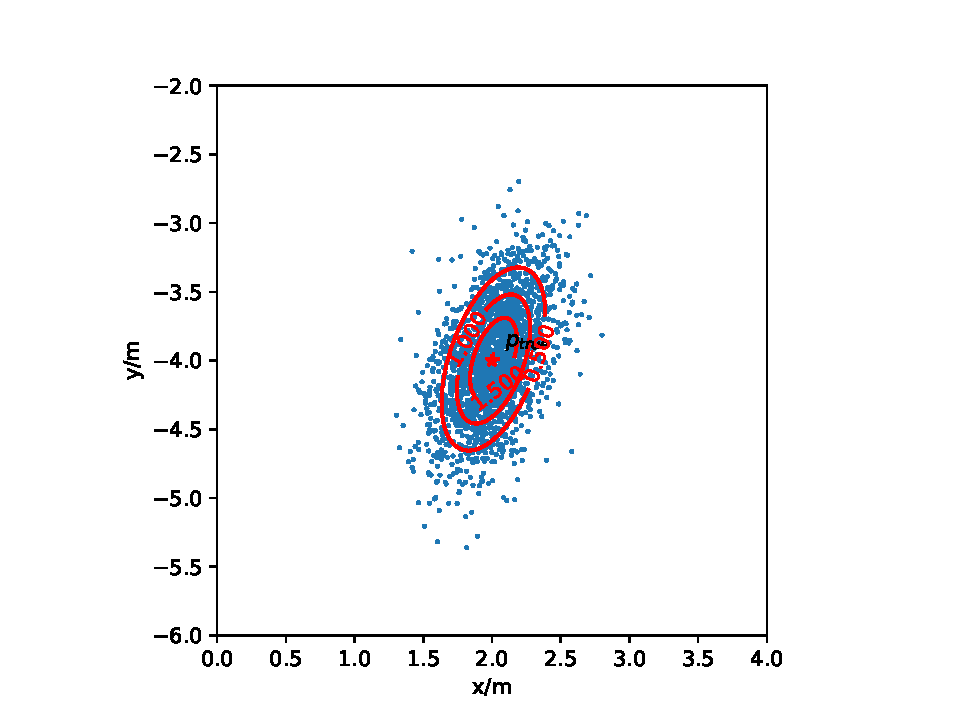
\includegraphics[width=.5\textwidth]{./Figures/scenario2_gausscont_big_withoutexp.pdf}
        }{%
        \caption{Scenario 2 without the exponential distributed anchor}%
        \label{fig:scenario2_gausscont_big_withexp}
		}
		\capbtabbox{%
  		\begin{tabular}{c|c} 
  		0,05175 & 0,04369 \\ \hline
  		0,04369 & 0,16122 \\ 
 		\end{tabular}
		}{%
 		\caption{Covariance matrix}%
		}
		\end{floatrow}
		\end{figure}
		
        Omitting the exponential anchor the variance is still bigger than in scenario 2 although the single estimations are more evenly distributed around the mean value which is also very close to the true position. Overall, the measurement is better without the exponential anchor.
        
	    \begin{figure}[hbt!]
        \begin{floatrow}
        \ffigbox{%
        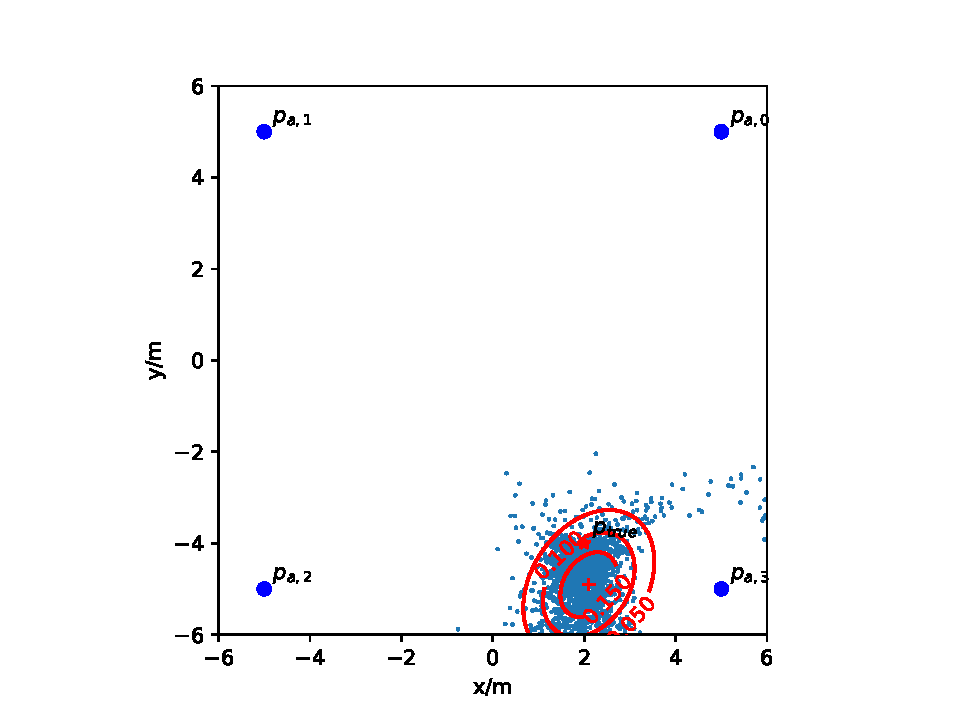
\includegraphics[width=.5\textwidth]{./Figures/scenario3_gausscont_small_ls.pdf}
        }{%
        \caption{Gaussian distribution of scenario 3}%
        \label{fig:scenario3_gausscont_small_ls}
		}
		\capbtabbox{%
  		\begin{tabular}{c|c} 
  		0,73497 & 0,25884 \\ \hline
  		0,25884 & 0,98659 \\ 
 		\end{tabular}
		}{%
 		\caption{Covariance matrix}%
		}
		\end{floatrow}
		\end{figure}
	
        The density function of scenario 3 is also computed by a general covariance matrix with bigger values in all dimensions. Therefore the point estimation is not precise and the variance around the mean value is very high.
        
        \newpage
        
        \begin{figure}[hbt!]
            \centering
            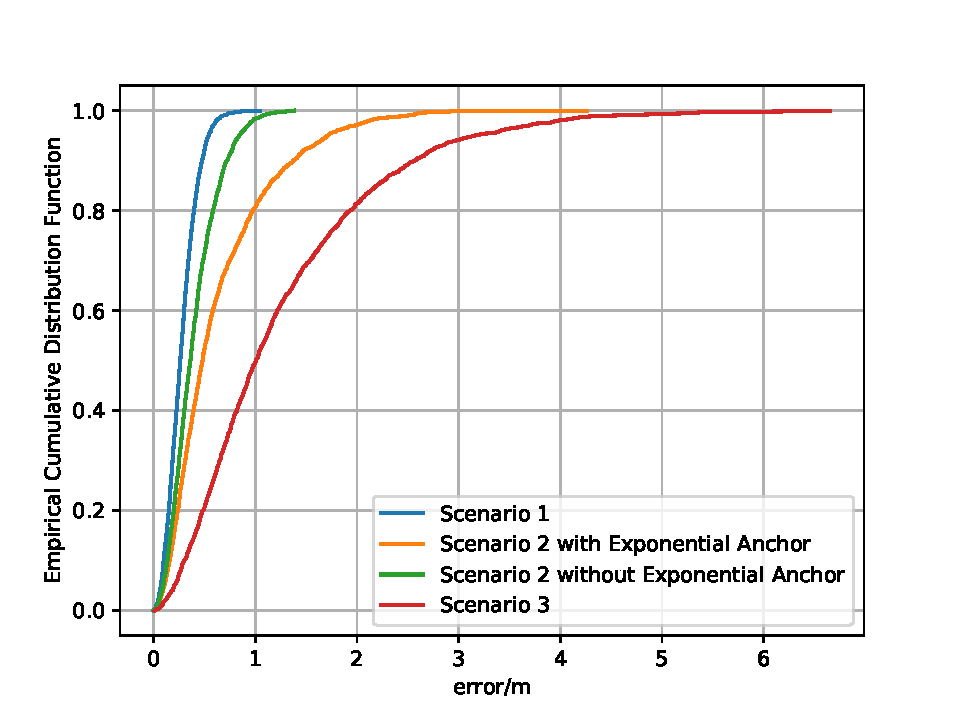
\includegraphics[width=\textwidth]{./Figures/All_ecdf_ls.pdf}
            \caption{Gaussian distribution of scenario 3}
            \label{fig:All_ecdf_ls}
        \end{figure}
        
        The cumulative distribution functions of the position errors emphasize our finding that the Gauss-Newton Algorithm is optimized for Gauss-distributed data sets. That is why scenario 1 delivers the best performance with a very low maximum error. Only using the three Gaussian anchors in scenario 2 leads to a similar cumulative distribution function with a slightly bigger maximum error. Taking the exponential anchor into account the maximum error greatly increases but 90\% of all errors are still smaller than the previous maximum error. Scenario 3 has the worst performance with  larger errors overall and by far the biggest maximum error.

\end{itemize}


\subsection{Numerical Maximum Likelihood Estimation of the Position}
\subsubsection{Single Measurement}

\begin{itemize}
\item The numerical maximum likelihood estimate is computed by finding the maximum of the joint likelihood of all anchors evaluated within a 2D-grid enclosed by the anchors. Because of the i.i.d.-assumption the joint likelihood can be calculated as the product of all individual exponential likelihoods:

\begin{align*}
p(\mathbf{\tilde{d}}_n(\mathbf{p})|\mathbf{p}) = 
\begin{cases}
\displaystyle \prod_{i=0}^{N_A-1} p(\tilde{d}_n(a_i,\mathbf{p})|\mathbf{p})\text{,}	& 	\; \text{if } \tilde{d}_n(a_i,\mathbf{p}) \geq d (a_i,\mathbf{p}) \; \forall i \\
\; 0 	&	\; \text{else}
\end{cases}
\end{align*} 

\begin{figure}[h]
\centering
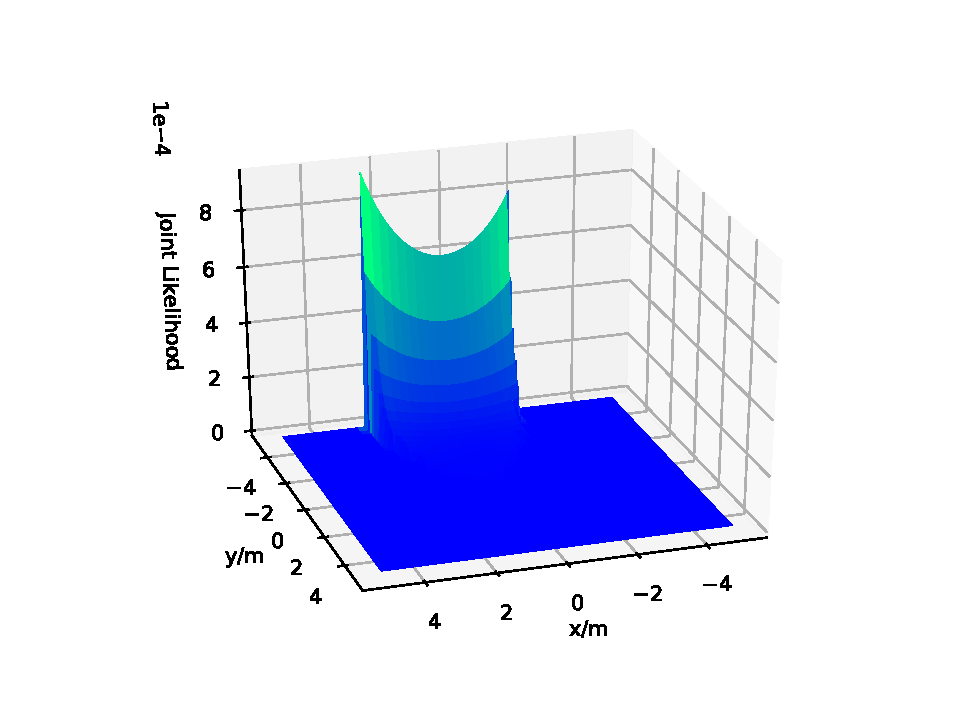
\includegraphics[width=0.9\textwidth]{./Figures/scenario3_grid_nml.pdf}
\caption{$p(\mathbf{\tilde{d}}_0(\mathbf{p})|\mathbf{p})$ evaluated within a 2D-grid enclosed by the anchors.}
\label{fig:scenario3_grid_nml}
\end{figure}

\item Because of its nonlinearity the joint likelihood function of the first sample $n=0$ has two local maxima (s. figure \ref{fig:scenario3_grid_nml}). If we used a gradient ascent algorithm with a random starting position, it would stop once it reaches any of them, possibly leading to a false estimation of the position, if the found maximum is not global.\\

\item The found maximum at $\mathbf{p}_{0,NML} = \left[ 2.5, -5 \right]$ is not at the true position. This is because the estimation is solely based on the noisy distance measurements $\mathbf{\tilde{d}}_0$: Within the grid the likelihood for each anchor $p(\tilde{d}_0(a_i,\mathbf{p})|\mathbf{p})$ is maximised on a circular arc with radius $\tilde{d}_0(a_i,\mathbf{p})$  and center $a_i$. The joint likelihood is nonzero within the area enclosed by both the grid borders and all arcs. Its maximum is at a point within this area as close as possible to all arcs - e.g. at the intersection of two arcs in close vicinity to the remaining ones - but because of the noisiness of the data and the restrictions of the grid, this is not necessarily the true position.
\end{itemize}

\subsubsection{Multiple Measurements}

\begin{itemize}
\item Both error mean $\mu_e$ and variance $\sigma^2_e$ of the NML estimation are much smaller than the corresponding parameters of the LS estimation (s. table \ref{tab:scen3_mean_var}). In figure \ref{fig:scenario3_ecdf_all} a lower maximum error of ca. 5.6m is visible with 90\% of all estimates having an error < 1.5m, which is an improvement over the LS errors. The cloud of position estimates displayed in the scatter-plot (s. figure \ref{fig:scenario3_gausscont_nml}) just below $\mathbf{p_{true}}$ is denser than the LS one but is truncated by the bottom grid border. There are also many outliers near the bottom and right grid borders which make the distribution seem even less Gaussian than the the LS results and cause the Gaussian-contour to be more tilted, indicating that the position estimate coordinates $x$ and $y$ are not statistically independent. 

\begin{figure}
\begin{subfigure}{\textwidth}
\centering
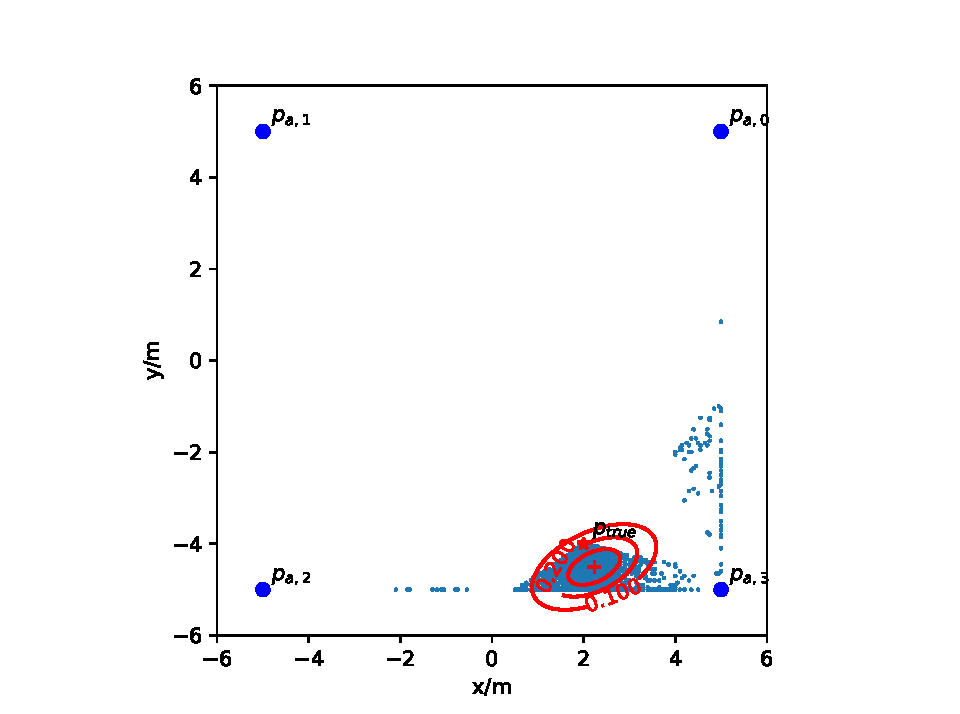
\includegraphics[width=\textwidth]{./figures/scenario3_gausscont_small_nml.pdf}
\caption{Full view of scatter plot.}
\end{subfigure}

\begin{subfigure}{\textwidth}
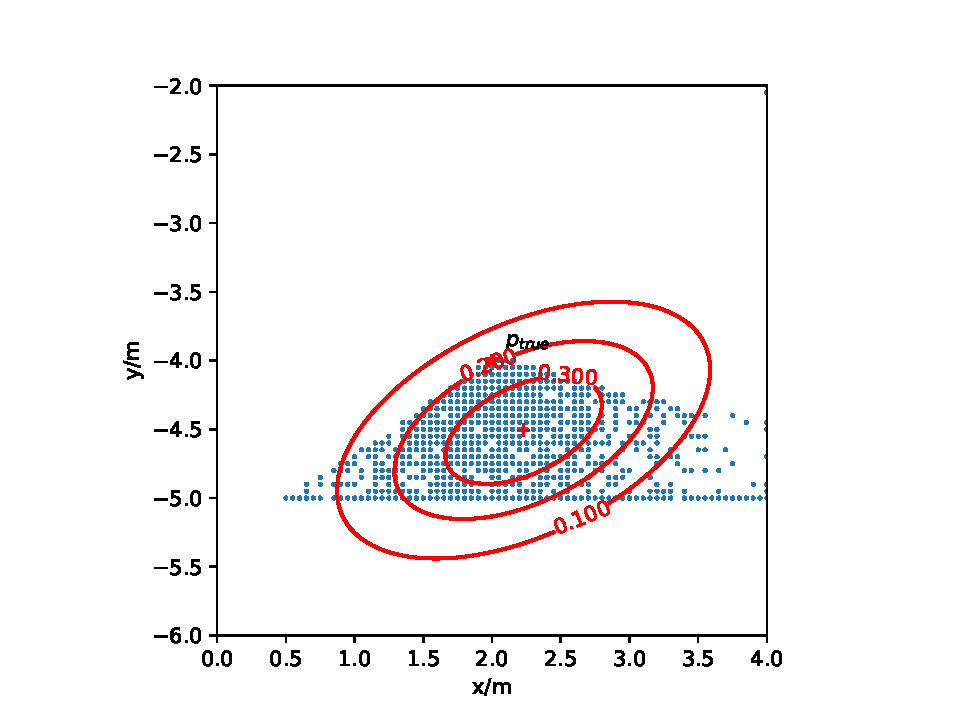
\includegraphics[width=\textwidth]{./figures/scenario3_gausscont_big_nml.pdf}
\caption{Detailed view centered on $\mathbf{p_{true}}$.}
\end{subfigure}
\caption{Scatter plot of NML-estimated positions with Gaussian-contour.}
\label{fig:scenario3_gausscont_nml}
\end{figure}


\item Of course this comparison is not very fair, since we are only looking at maxima within the grid enclosed by the anchors. This prevents position estimates with larger error values - e.g. estimates below $y=-5$ as in the LS-case - which explains the smaller error parameters. But this also means that the numerical approach confined by the grid borders and its limited resolution is not truly a Maximum Likelihood Estimator, as we can not find the actual maximum of the joint likelihood for all samples.

\item
The prior knowledge used for the Bayes estimator greatly enhances the accuracy. Here the error mean $\mu_e$ is almost half as big as the LS one, the error variance $\sigma^2_e$ is cut down to almost one tenth of the LS result (s. table \ref{tab:scen3_mean_var}). Looking at figure \ref{fig:scenario3_ecdf_all} the Bayes estimator is a big improvement over the other approaches, the maximum error being only 1.2m. This is also visible in the scatter-plot (s. figure \ref{fig:scenario3_gausscont_bayes}), which shows a very dense estimate-cluster with no outliers. However it is still not centred on $\mathbf{p_{true}}$ but on about the same mean estimate as the NML estimation. The Gaussian-contour is not tilted and (because the cluster is slightly truncated by the bottom grid border) almost circular, indicating stochastically independent estimate coordinates with similar variance.


\end{itemize}

\begin{table}[h]
\centering
\begin{tabular}{l||c||c||c|}
\cline{2-4}
                                                   & Least-Squares & Numerical Maximum Likelihood & Bayes  \\ \hline \hline
\multicolumn{1}{|l||}{Error mean $\mu_e$}           & 1.265              & 0.915                       & 0.680 \\ \hline
\multicolumn{1}{|l||}{Error variance $\sigma^2_e$} &  0.939 & 0.489                       & 0.095 \\ \hline
\end{tabular}
\caption{Error-mean and -variance of Least-Squares-, Numerical Maximum Likelihood- and Bayes-Estimation.}
\label{tab:scen3_mean_var}
\end{table}

\begin{figure}[h]
\centering
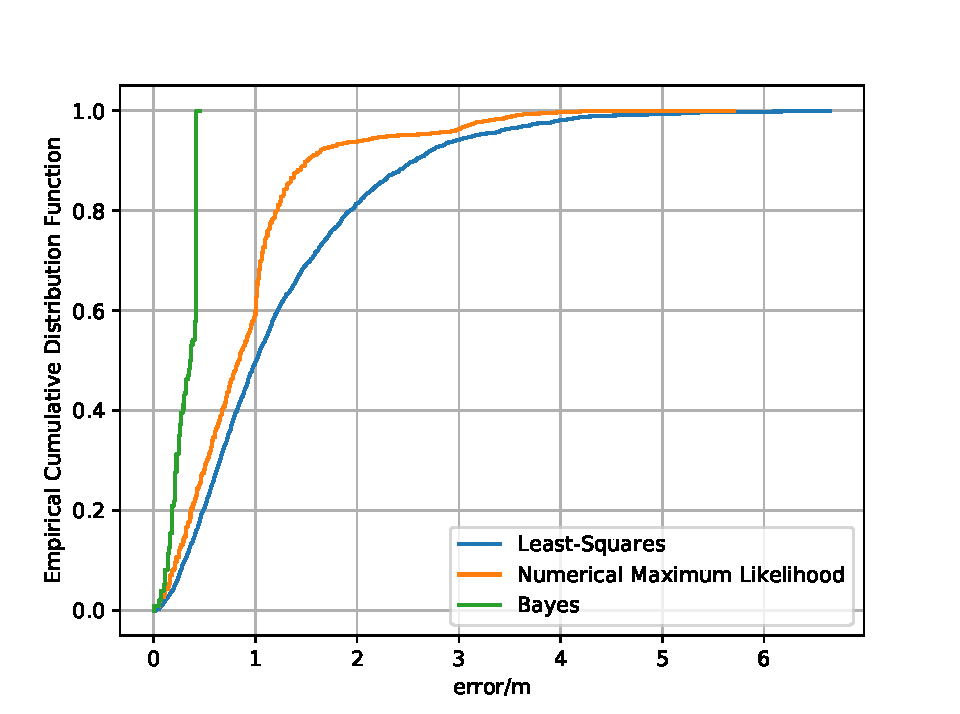
\includegraphics[width=0.8\textwidth]{./Figures/scenario3_ecdf_all.pdf}
\caption{ECDF of Least-Squares-, Numerical Maximum Likelihood- and Bayes-Estimation.}
\label{fig:scenario3_ecdf_all}
\end{figure}

\begin{figure}[h]
\begin{subfigure}{\textwidth}
\centering
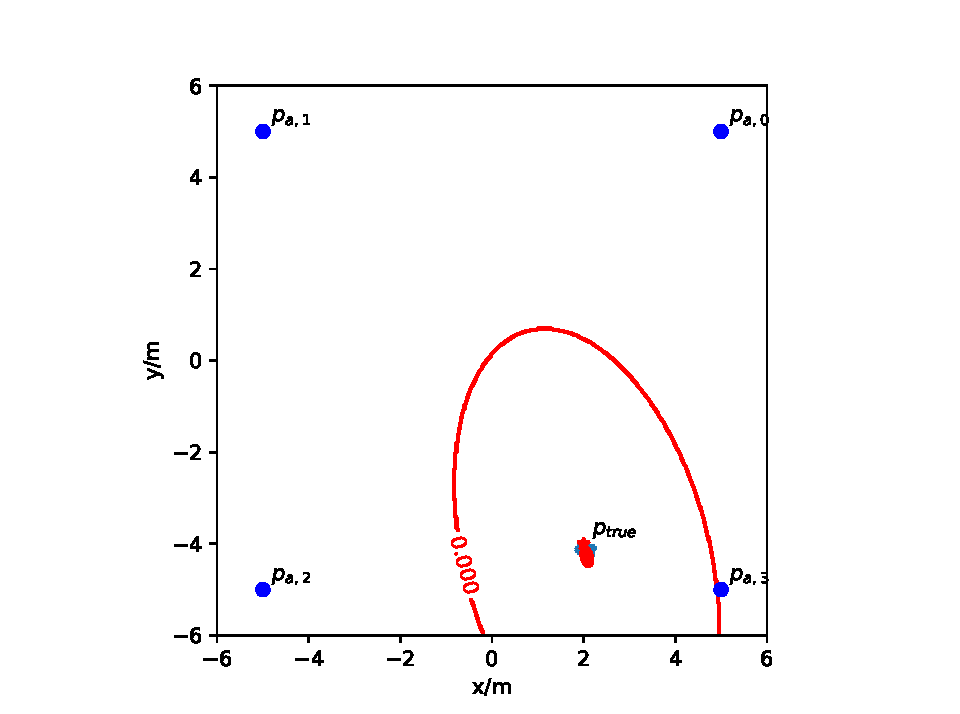
\includegraphics[width=\textwidth]{./figures/scenario3_gausscont_small_bayes.pdf}
\caption{Full view of scatter plot.}
\end{subfigure}

\begin{subfigure}{\textwidth}
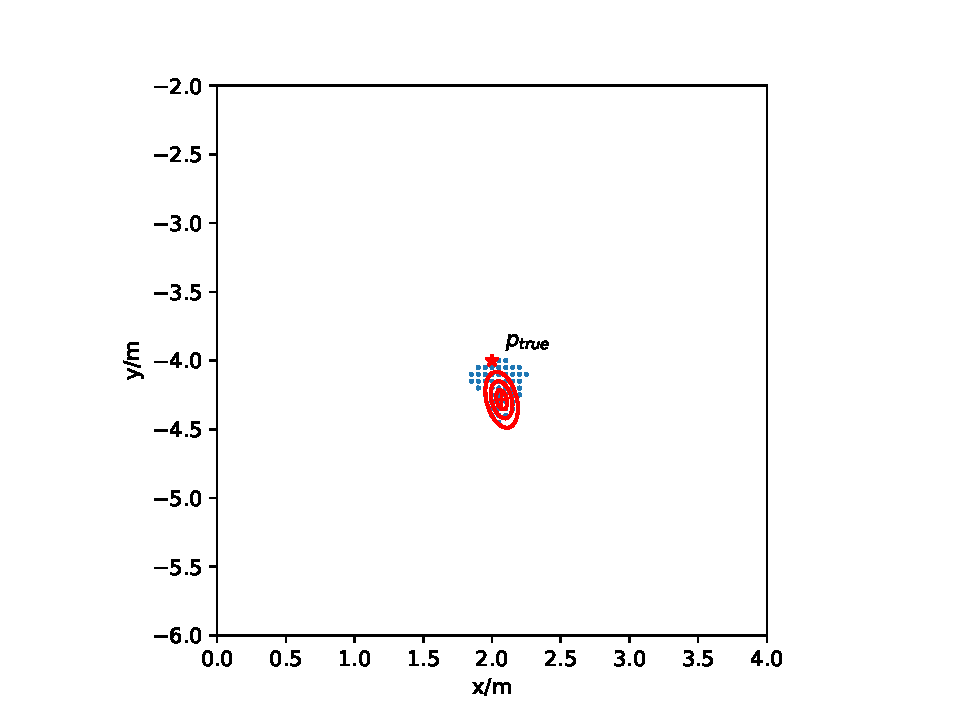
\includegraphics[width=\textwidth]{./figures/scenario3_gausscont_big_bayes.pdf}
\caption{Detailed view centered on $\mathbf{p_{true}}$.}
\end{subfigure}
\caption{Scatter plot of Bayes-estimated positions with Gaussian-contour.}
\label{fig:scenario3_gausscont_bayes}
\end{figure}

\end{document}